
\documentclass[11pt,oneside]{article} 

\usepackage{a4wide}

\usepackage{amsmath}
\usepackage{color}
%\usepackage{natbib} % kills arxiv 
\usepackage{framed}
%\usepackage{cite}
\usepackage{tikz}
\usepackage{tikz-cd}

% http://www.maths.qmul.ac.uk/~mf/genyoungtabtikz.sty
\usepackage[vcentermath]{genyoungtabtikz}
\Yboxdim{8pt}
%\Ylinethick{1pt}

\RequirePackage{amsmath}
\RequirePackage{amssymb}
\RequirePackage{amsthm}

%\RequirePackage{algorithmic}
%\RequirePackage{algorithm}
%\RequirePackage{theorem}
%\RequirePackage{eucal}
\RequirePackage{color}
\RequirePackage{url}
\RequirePackage{mdwlist}

\RequirePackage{rotating}


\RequirePackage[all]{xy}
%\_CompileMatrices
%\RequirePackage{hyperref}
\RequirePackage{graphicx}
%\RequirePackage[dvips]{geometry}

\usepackage{xcolor}
%\usepackage{amsmath,amsfonts,amssymb}
\usepackage{graphicx}
\usepackage[caption=false]{subfig}
\usepackage{enumerate}
\usepackage{mathrsfs}
\usepackage{bbm}

% -------------- Commands ----------------------

\makeatletter
\newcommand{\verbatimfont}[1]{\renewcommand{\verbatim@font}{\ttfamily#1}}
\makeatother

\newcommand{\Eref}[1]{(\ref{#1})}
\newcommand{\Fref}[1]{Fig.~\ref{#1}}
%\newcommand{\Aref}[1]{Appendix~\ref{#1}}
\newcommand{\SRef}[1]{Section~\ref{#1}}

\newcommand{\todo}[1]{\ \textcolor{red}{\{#1\}}\ }

\newcommand{\Aut}{\mathrm{Aut}}
\newcommand{\Hom}{\mathrm{Hom}}
%\newcommand{\hom}{\mathrm{hom}} % internal hom ?
\newcommand{\Stab}{\mathrm{Stab}}
\newcommand{\Fix}{\mathrm{Fix}}
\newcommand{\Orbit}{\mathrm{Orbit}}
\newcommand{\Ker}{\mathrm{Ker}}
\newcommand{\Image}{\mathrm{Im}}
\newcommand{\Dim}{\mathrm{Dim}}
\newcommand{\Complex}{\mathbb{C}}
\newcommand{\Integer}{\mathbb{Z}}
\newcommand{\Natural}{\mathbb{N}}

\newcommand{\GL}{\mathrm{GL}}
\newcommand{\SL}{\mathrm{SL}}
\newcommand{\PGL}{\mathrm{PGL}}
\newcommand{\Field}{\mathbb{F}}

% Lemma, proof, theorem, etc.
\newcommand\nounderline[1]{ #1} 
\newcommand\dodef[1]{\vskip 5pt \noindent{\bf \underline{Definition #1.}\ }}
\newcommand\dolemma[1]{\vskip 5pt \noindent{\bf \underline{Lemma #1.}\ }}
\newcommand\doproposition[1]{\vskip 5pt \noindent {\bf \underline{Proposition #1.}\ }}
\newcommand\dotheorem[1]{\vskip 5pt \noindent {\bf \underline{Theorem #1.}\ }}
\newcommand\docorollary[1]{\vskip 5pt \noindent {\bf \underline{Corollary #1.}\ }}
\newcommand\doexample[1]{\vskip 5pt \noindent {\bf \underline{Example #1.}\ }}
\newcommand\doproof{\vskip 5pt \noindent{\bf \nounderline{Proof:}\ }}

\newcommand\tombstone{\rule{.36em}{2ex}\vskip 5pt}

\newcounter{numitem}
\newcommand{\numlabel}[1]{\refstepcounter{numitem}\thenumitem\label{#1}}
\newcommand{\numitem}{\refstepcounter{numitem}\thenumitem}

% Categories
\newcommand{\Set}{\mathbf{Set}}
\newcommand{\FinSet}{\mathbf{FinSet}}
\newcommand{\GSet}{\mathbf{GSet}}
\newcommand{\GRep}{\mathbf{GRep}}

\newcommand{\thinplus}{\!+\!}

\renewcommand{\arraystretch}{1.2}

\newcommand{\tensor}{\otimes}



\title{Sketching Algebraic Groups}

\author{Sijato Budotr}

\date{\today}

\flushbottom

\begin{document}

\maketitle

%\begin{abstract}
%\end{abstract}

%\tableofcontents

%\doublespacing
%\onehalfspacing

\section*{Representation theory of $S_n$}

% https://golem.ph.utexas.edu/category/2007/04/schur_functors.html#c008943
%    There are two Schur functors, corresponding to the partitions
%    (2) and (1,1); I’ll denote them by S2S^2 and S1,1S^{1,1}.
%    The definition (according to Fulton) is that S2(V)S^2(V)
%    is the quotient of V⊗2V^{\otimes 2} by the subspace spanned
%    by expressions of the form u⊗v−v⊗uu \otimes v - v \otimes
%    u; the definition of S1,1(V)S^{1,1}(V) is the quotient
%    of V⊗2V^{\otimes 2} by the subspace spanned by elements
%    of the forms u⊗uu \otimes u and u⊗v+v⊗uu \otimes v +
%    v \otimes u. It is easy enough to see how S2S^2 and S1,1S^{1,1}
%    should act on morphisms.
%    
%    Now, any construction involving quotients should have
%    a dual construction involving subspaces. So let S2(V)S_2(V)
%    be the kernel of V⊗2→S1,1(V)V^{\otimes 2} \to S^{1,1}(V)
%    and let S1,1(V)S_{1,1}(V) be the kernel of V⊗2→S2(V)V^{\otimes
%    2} \to S^2(V). S2S_2 and S1,1S_{1,1} are also functors
%    in a clear way.


We have the decomposition
$$
    V^{\tensor 2} \cong \yng(2)(V) \oplus \yng(1,1)(V)
$$
or, just counting dimensions:
\begin{center}
\begin{tabular}{cccc}
V  &    $V^{\otimes 2}$ &  $\yng(2)(V)$  &  $\yng(1,1)(V)$   \\
    \hline
0&    0  &  0   &  0   \\
1&    1  &  1   &  0   \\
2&    4  &  3   &  1   \\
3&    9  &  6   &  3   \\
4&    16  &  10   &  6   \\
... &  &     &     \\
\end{tabular}
\end{center}

Going to a third tensor power, we get
$$
    V^{\tensor 3} \cong \yng(3)(V) \oplus 
        2\cdot \yng(1,2)(V) \oplus \yng(1,1,1)(V).
$$
In general these tensor powers $V^{\tensor n}$ decompose as
a sum over Young diagrams $\lambda$ with number of boxes $|\lambda|=n$,
and with multiplicity $m_\lambda$:
$$
V^{\tensor n} \cong \bigoplus_{|\lambda|=n}
    m_\lambda\cdot \lambda(V).
$$

A categorified binomial theorem (\cite{Brandenburg2014} Lemma 3.2.1).
Given finite dimensional vector spaces $V,W$ and $n\in\Natural$,
$$
    (V\oplus W)^{\tensor n} \cong 
        \bigoplus_{m=0}^n
        {n\choose m}\cdot
        V^{\tensor m}\tensor W^{\tensor (n-m)}.
$$
Now we combine this binomial theorem with the
observations above, any Young diagram $\lambda$ with $n$ boxes
we have a map:
$$
    \lambda(V\oplus W) \to 
        \bigoplus_{m=0}^n
        {n\choose m}\cdot
        V^{\tensor m}\tensor W^{\tensor (n-m)}.
$$
So there should be a binomial formula for each Young diagram.
Here are two examples:
\begin{align*}
\yng(1,2)(V\oplus W) 
\cong\ \ \ \   & \yng(1,2)(V)\tensor\phi(W) \\
\oplus\ & \yng(2)(V)  \tensor\yng(1)(W)  \\
\oplus\ & \yng(1,1)(V)  \tensor\yng(1)(W)  \\
\oplus\ & \yng(1)(V)  \tensor\yng(2)(W)  \\
\oplus\ & \yng(1)(V)  \tensor\yng(1,1)(W)  \\
\oplus\ & \phi(V)  \tensor\yng(1,2)(W) .
\end{align*}
The empty Young diagram is $\phi$ and $\phi(V)\cong \Complex.$
Another example:
\begin{align*}
\yng(2,2)(V\oplus W) 
\cong\ \ \ \   & \yng(2,2)(V)\tensor\phi(W) \\
\oplus\ & \yng(1,2)(V)  \tensor\yng(1)(W)  \\
\oplus\ & \yng(2)(V)  \tensor\yng(2)(W)  \\
\oplus\ & \yng(1,1)(V)  \tensor\yng(1,1)(W)  \\
\oplus\ & \yng(1)(V)  \tensor\yng(1,2)(W)  \\
\oplus\ & \phi(V)  \tensor\yng(2,2)(W) .
\end{align*}

\section*{Representation theory of GL(n)}

We are considering algebraic groups over the field of
complex numbers, and the monoidal category of representations of 
these groups.

\subsection*{GL(1)}

TODO

\subsection*{GL(2)}

This pair of short exact sequences are key
to understanding the following:
\[
\begin{tikzcd}
    &  
    \SL(2) \arrow[rightarrowtail]{d}\arrow[two heads]{dr}{\mathrm{2-to-1}} &  \\
    \GL(1) \arrow[rightarrowtail]{r}{\mathrm{diag}} 
           \arrow[two heads]{dr}[below,left]{\mathrm{2-to-1\ }}  &  
    \GL(2) \arrow[two heads]{r}\arrow[two heads]{d}{\mathrm{det}}  &  \PGL(2)     \\
    &  \GL(1)             &     \\
\end{tikzcd}
\]


We label the irreducible represenations of SL(2) by
Young diagrams with one row:
\begin{center}
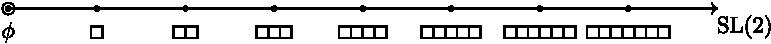
\includegraphics[]{images/sl2.pdf}
\end{center}

Within these, we have a subcategory of represenations of PGL(2):
\begin{center}
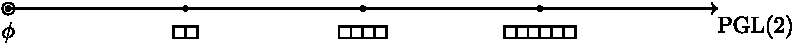
\includegraphics[]{images/pgl2.pdf}
\end{center}

The irreducible represenations of GL(2) look like this:
\begin{center}
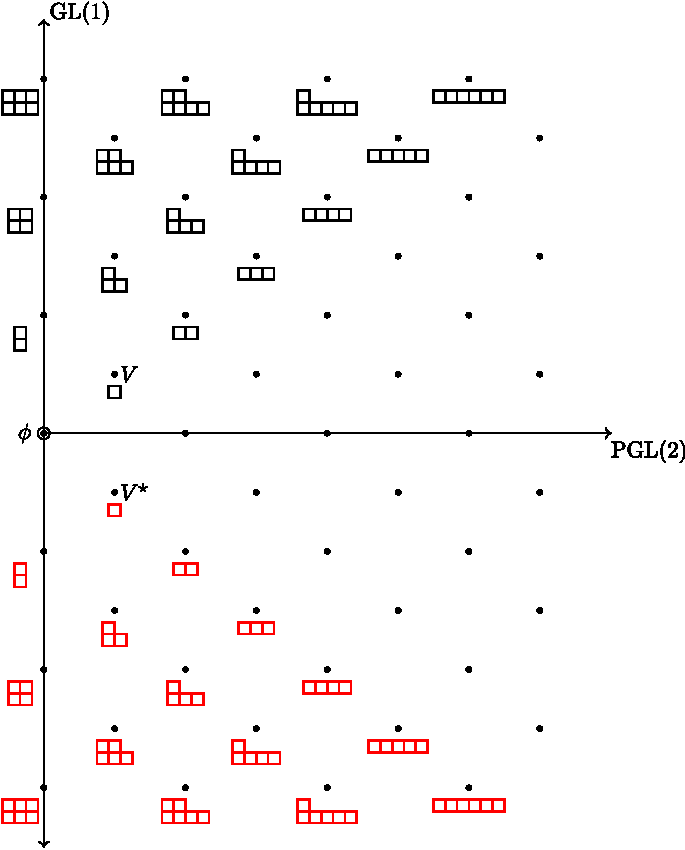
\includegraphics[scale=0.8]{images/gl2.pdf}
\end{center}
Where we have labelled the tautological (natural) represenation as $V$
and its dual as $V^{\star}.$

\subsection*{GL(3)}

\[
\begin{tikzcd}
    &  
    \SL(3) \arrow[rightarrowtail]{d}\arrow[two heads]{dr}{\mathrm{3-to-1}} &  \\
    \GL(1) \arrow[rightarrowtail]{r}{\mathrm{diag}} 
           \arrow[two heads]{dr}[below,left]{\mathrm{3-to-1\ }}  &  
    \GL(3) \arrow[two heads]{r}\arrow[two heads]{d}{\mathrm{det}}  &  \PGL(3)     \\
    &  \GL(1)             &     \\
\end{tikzcd}
\]

We start with a picture of the $\SL(3)$ kaleidoscope:
\begin{center}
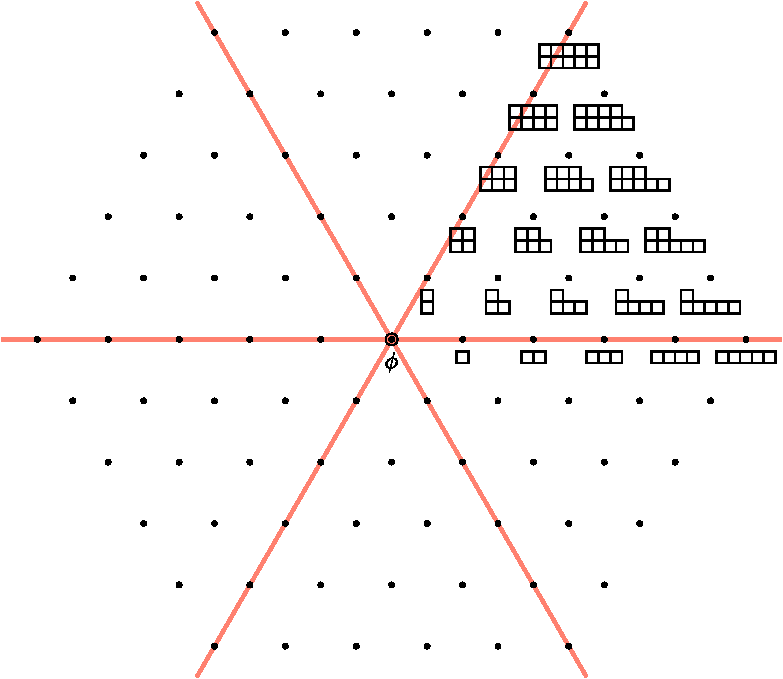
\includegraphics[scale=0.8]{images/sl3.pdf}
\end{center}

The epimorphism SL(3)$\to$PGL(3) is a 3-to-1 map,
and so we find the irreps of PGL(3) as an index 3 
sublattice of the SL(3) kaleidoscope:
\begin{center}
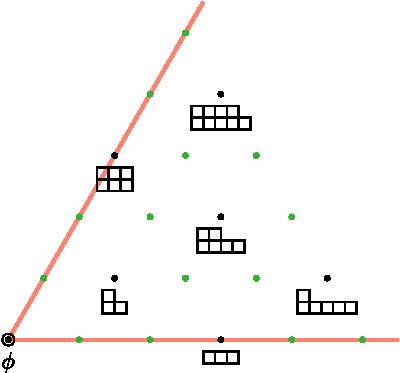
\includegraphics[scale=0.8]{images/pgl3.pdf}
\end{center}

The positive levels of $\GL(3)$:
\begin{center}
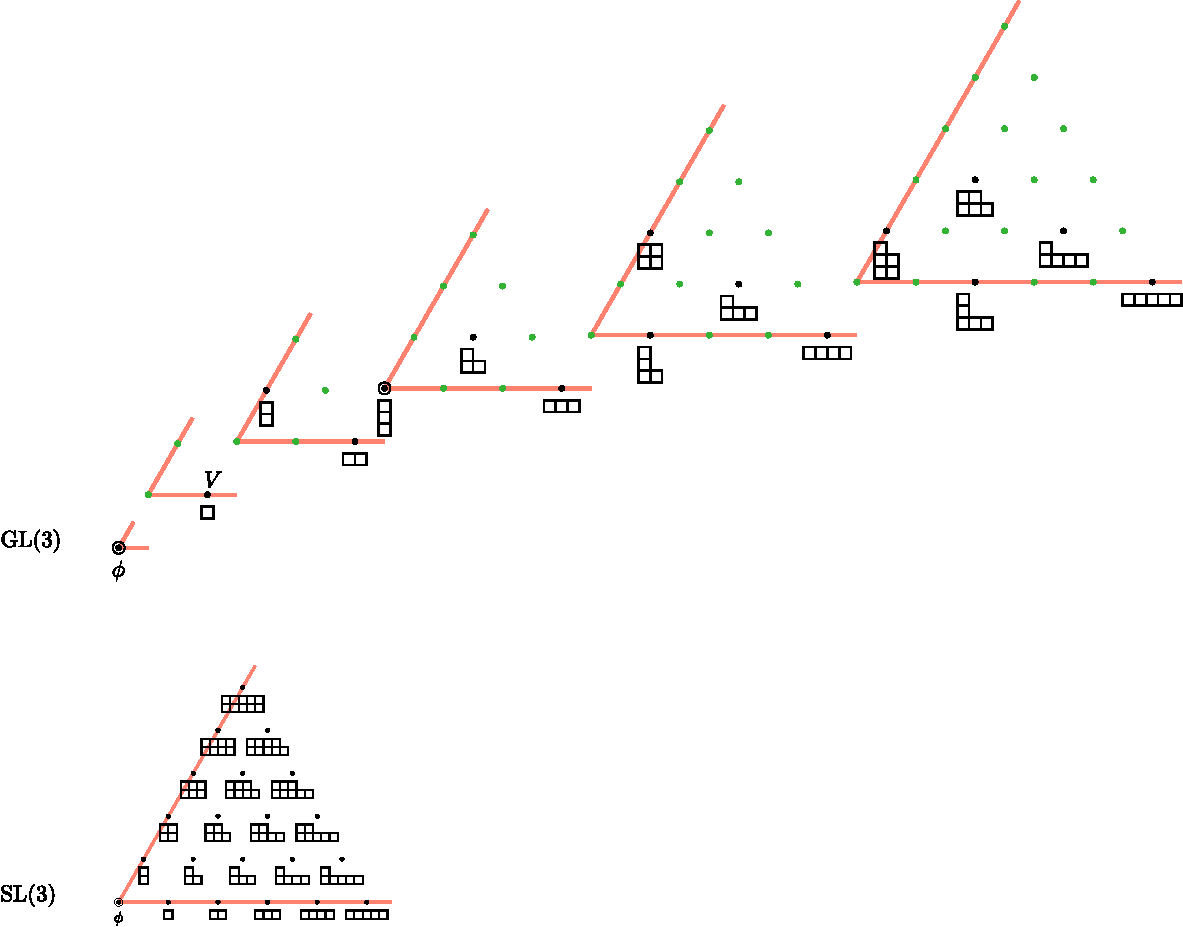
\includegraphics[scale=0.6]{images/gl3.pdf}
\end{center}

\bibliography{refs2}{}
\bibliographystyle{abbrv}

\end{document}
